\chapter{Variational Bayesian Inference} \label{sec:vi}

\section{Introduction}

Variational Bayesian inference is a generic term for a set of algorithms that cast the problem of Bayesian inference as an optimisation problem, and is commonly referred to as just \textit{variational inference} (VI). The basic idea behind this framework is simple, but many different approaches exist, each with their own practical (dis)advantages.
\\
In this chapter an introduction to the theoretical background of variational inference will be provided. Following this, we will see several different VI algorithms and provide a simple comparison. We are most interested in those variants of VI that do not require excessive mathematical derivation from the end user. The chapter will be closed with an overview of the use of VI in the field of bioinformatics.

\section{Variational inference \parencite{vi-review, vi}}

\par Variational inference (VI) is a Bayesian inference technique that attempts to find a distribution that approximates the true posterior. In VI, there is no sampling - as in MCMC - but instead the problem is modelled as an optimisation.
\medskip
\par The inference problem at hand is to calculate the conditional density $p(\bm{{z}}|\bm{x})$ of the latent variables $\bm{z}$ for a given set of observed variables $\bm{x}$.
    
    \begin{equation}
        p(\bm{z} | \bm{x}) = \frac{p(\bm{x}, \bm{z})}{p(\bm{x})} = \frac{p(\bm{z})p(\bm{x}|\bm{z})}{p(\bm{x})}
    \end{equation}
\\
In most cases the evidence $p(\bm{x})$ will be unknown, being either mathematically intractable or so computationally expensive as to be unavailable in practice.


\subsection{Variational families}

\par Generally, an approximate distribution $q$ is chosen out of a variational family of distributions $\mathcal{Q}$. For reasons of mathematical and computational simplicity the mean-field variational family is most commonly used, as a more complex variational family increases the complexity of the optimisation problem.
\\
The most important characteristic of the mean-field variational family is that all latent variables $z_i$ are independent, and each is modelled by a separate factor $q_i$ (see Equation \ref{eq:mean-field}).

\begin{equation}
    \label{eq:mean-field}
    q(\bm{z}) = \prod^{N}_{i=1}{q_i(z_i)}
\end{equation}
    

\subsection{The evidence lower bound (ELBO) \parencite{vi-review}}

\paragraph{}
{
    The main principle behind variational inference is to model the inference problem as an optimisation problem, and as such we require a metric to optimise. A good candidate for this is the Kullback–Leibler divergence \parencite{KL}, which is a measure of difference between two probability distributions. The KL divergence is defined as in Equation \ref{eq:KL}, where the expectation is taken with respect to $q(\bm{z})$. It is evident from the definition that this metric is asymmetric.
    
    \begin{equation}
        \label{eq:KL}
            \begin{split}
            \mathrm{KL} \big( q(\bm{z})\, ||\, p(\bm{z}|\bm{x}) \big) 
            = & \  
            \mathbb{E}_{q(\bm{z})} \big[ \mathrm{log} \: q(\bm{z}) - 
            \mathrm{log} \: p(\bm{z}|\bm{x}) \big] \\
            = & \ 
            \mathbb{E}_{q(\bm{z})} \big[ \mathrm{log} \: q(\bm{z}) \big] - 
            \mathbb{E}_{q(\bm{z})} \big[ \mathrm{log} \: p(\bm{z}|\bm{x}) \big] \\
            = & \
            \mathbb{E}_{q(\bm{z})} \big[ \mathrm{log} \: q(\bm{z}) \big] - 
            \mathbb{E}_{q(\bm{z})} \big[ \mathrm{log} \: p(\bm{z},\bm{x}) \big] + 
            \mathbb{E}_{q(\bm{z})} \big[ \mathrm{log} \: p(\bm{x}) \big] \\
            = & \
            \mathbb{E}_{q(\bm{z})} \big[ \mathrm{log} \: q(\bm{z}) \big] - 
            \mathbb{E}_{q(\bm{z})} \big[ \mathrm{log} \: p(\bm{z},\bm{x}) \big] + 
            \mathrm{log} \: p(\bm{x})
        \end{split}
    \end{equation}
    \\
    The resulting optimisation of the KL divergence can be written as follows (Equation \ref{eq:argmin-KL}):
    
    \begin{equation}
        \label{eq:argmin-KL}
        q^*(\bm{z}) = \underset{q(\bm{z}) \in \mathcal{Q}} 
        {\mathrm{argmin}} \; \mathrm{KL} \big( q(\bm{z})||p(\bm{z}|\bm{x}) \big)
    \end{equation}
    \\
    The formula for the KL divergence is dependent on the \textit{marginal likelihood} (also called the \textit{evidence}) $p(\bm{x})$ which is intractable. In practice another metric related to the KL divergence, but not dependent on the evidence, will be used: the evidence lower bound (ELBO) as defined in Equation \ref{eq:elbo}.
    \\
    
    \begin{equation}
        \label{eq:elbo}
        \begin{split}
            \mathrm{ELBO}(q)
            = &  
            \mathbb{E}_{q(\bm{z})} \big[ \mathrm{log} \: p(\bm{z},\bm{x}) \big] -
            \mathbb{E}_{q(\bm{z})} \big[ \mathrm{log} \: q(\bm{z}) \big] \\
            = & 
            \mathbb{E}_{q(\bm{z})} \big[ \mathrm{log} \: p(\bm{z}) + \mathrm{log} \: p(\bm{x}|\bm{z}) \big] - 
            \mathbb{E}_{q(\bm{z})} \big[ \mathrm{log} \: q(\bm{z}) \big] \\
        \end{split}
    \end{equation}
    \\ The ELBO is, as the name suggests, a lower bound for the evidence: the $ \mathrm{log} \: p(\bm{x)}$ is always smaller than the ELBO for any $q(\bm{z)}$. It can also be written as 
    
    \begin{equation}
       \mathrm{ELBO}(q)
        = 
        \mathrm{log} \: p(\bm{x}) - \mathrm{KL} \big( q(\bm{z}) \, || \, p(\bm{z}|\bm{x}) \big)
        .
    \end{equation}
    \\
    Because the KL divergence is positive by definition \parencite{KL}, it is evident that the ELBO is indeed a lower bound for $\mathrm{log} \, p(\bm{x})$. Equation \ref{eq:elbo} shows that the ELBO is dependent only on known probability densities: the prior $p(\bm{z})$, the likelihood $p(\bm{x}|\bm{z})$ and the variational distribution $q(\bm{z})$. The ELBO is at its maximum when the KL divergence is minimal; the argmin problem has been transformed into the following argmax problem (Equation \ref{eq:elbo-max}).
    
    \begin{equation}
        \label{eq:elbo-max}
        q^*(\bm{z}) = \underset{q(\bm{z}) \in \mathcal{Q}}{\mathrm{argmax}} \Big( \mathrm{ELBO} \big( q(\bm{z}) \big) \Big)
    \end{equation}
    \\
    In a typical optimisation problem it would now be possible to take the gradient of this expression and numerically reach the optimum through a gradient ascent method e.g. ADAM \parencite{ADAM}. However, in this case the problem is not so simple because we are working with potentially intractable expectations - depending on the model - inside the ELBO function.
    \\ 
    In Section \ref{sec:vi-methods} several VI methods will be discussed that each propose a way around this problem.
}


\subsection{Comparison with MCMC}

\par Blei et al. provide a brief comparison of VI and MCMC in their review paper \parencite{vi-review}, stating that MCMC methods are generally more computationally intensive than VI, and do not scale as well to large datasets. MCMC does guarantee that true posterior samples will eventually be produced, although it will often be computationally infeasible to ever reach that theoretical limit.
\\
We can broadly state that VI is suitable for data-driven applications with large (low-quality) datasets where an approximation of the true posterior is an acceptable result; or for applications where results are expected in real-time. Conversely, MCMC is preferred for manually curated small datasets, and when great accuracy is required. 
\\
Bioinformatics problems have traditionally been of the latter type, but the increasing availability of high-quality genomic data means that researchers are looking to perform larger studies.
\\
The phylogenetic problems studied in this thesis have small datasets and are conventionally solved with MCMC; however, these MCMC methods are too computationally intensive to be scaled to studies of large species trees.


\section{VI methods} \label{sec:vi-methods}

While there are dozens of VI methods that each optimise the ELBO function in different ways, it is possible to distinguish two main approaches to the problem. The first (e.g. CAVI) assumes that the expectation in the ELBO is tractable, and that parameter updates can be manually derived. The second approach (e.g. BBVI, ADVI) aims to find a noisy but unbiased (expected value is same as that of true gradient) estimator for the gradient $\nabla_{\lambda}\mathrm{ELBO}$, where $\lambda$ are the variational parameters.
\\
A third and wholly different take on variational optimisation is Stein Variational Gradient Descent (SVGD, see \ref{sec:svgd}) which is a sampling method that iterative updates a set of samples (called particles) until they approximate the true posterior density. This technique does not use the ELBO, nor does it require the specification of a variational family.

\subsection{Coordinate ascent variational inference (CAVI)} \label{sec:cavi}

The most straightforward method of variational inference is coordinate ascent \parencite{vi-review}, which involves calculating separate coordinate updates for each variational parameter and then performing gradient updates until convergence. In the CAVI algorithm (Algorithm \ref{alg:cavi}) an exponential variational family is assumed, and only one parameter is updated at a time, which requires the computation of the expectation $\mathbb{E}_{-i}$ which denotes the expectation in respect to all parameters except that one with index $i$.
\\
These coordinate updates have to be derived manually, which in many cases is impossible; the model may be mathematically intractable or we may be working with a black-box model of which part of the internal mathematics are unknown.
    
\medskip
\par In this thesis we study phylogenetic models for which the ELBO expectations are intractable, so CAVI can never be applied here. This method is, however, the fastest VI algorithm available, often several orders of magnitude faster than MCMC.


\subsubsection{Convergence testing}
Convergence of CAVI, and other VI methods described later in this section, is not always tested by evaluating the ELBO on the whole dataset at each iteration. This could be too computationally intensive; instead convergence is typically tested by evaluating the ELBO on a small held-out subset of the data that is only used for checking convergence and never to calculate the parameter updates. This held-out set is functionally equivalent to what would be called a "validation set" in machine learning contexts.



\begin{algorithm}
    \label{alg:cavi}
    \KwIn{model p(\bm{x}, \bm{z}), \mathrm{data} \; \bm{x}, \\
    \qquad \qquad variational density $q(\bm{z}) = \prod^{N}_{i=1}{q_i(z_i)}$}
    \KwOut{Optimised variational density $q^*(\bm{z})$}
    \While{ELBO not converged}{
        \For{each $q_i \in q$}{
            $q_i(z_i) \propto \mathrm{exp} \big\{ \mathbb{E}_{-i} [ \mathrm{log}p(z_i | \bm{z_{-i}}, \bm{x} ) ] \big\}$
        }
        Calculate ELBO($q$)
    }
    \Return{$q(\bm{z})$}
    \caption{Coordinate ascent variational inference (CAVI)}
\end{algorithm}



\subsection{Automatic differentiation variational inference (ADVI)} \label{sec:advi}

In practice the ELBO function is often intractable so that CAVI cannot be used. Some methods will apply specific conditions to the model and variational family, under which the ELBO can be calculated.
\\
Automatic differentiation variational inference (ADVI) is a technique that uses the following strategy in order to automate the variational inference optimisation:

\begin{itemize}
    \item First the latent variables of the model are transformed into real-space with a transformation $T$.
    
    \item A variational approximation is chosen that conforms to very specific requirements: either $q$ is a mean-field distribution made up of univariate Gaussians (Equation \ref{eq:mean-field-advi}), or it is a single N-dimensional multivariate ("full-rank") Gaussian (Equation \ref{eq:full-rank-advi}). In these equations $\bm \zeta$ are the latent model variables and $\bm \phi $ the variational parameters. In this thesis we will only discuss the univariate case; for a mathematical description of the multivariate case, we refer to the original paper by \cite{ADVI}.
    
    \item Finally, the optimisation process is performed in a generic way that applies to any differentiable probability model $p(\bm{\theta}, \bm{x})$. Gradients in the optimisation are calculated using \textit{automatic differentiation} (AD), which is a generic term for the process of automatically computing derivatives, typically by recursively applying the chain-rule to an expression \parencite{AD}. This means that if the model is known to be differentiable, the user can treat it as a black box. 
\end{itemize}


\begin{equation} 
    \label{eq:mean-field-advi}
    q(\bm{\zeta}; \bm{\phi}) = \sum^K_{i=1} \mathrm{Normal}(\mu_i, \sigma_i)
\end{equation}

\begin{equation}
    \label{eq:full-rank-advi}
    q(\bm{\zeta}; \bm{\phi}) = \mathrm{Normal(\bm{\zeta} \, | \bm{\mu}, \, \bm{\Sigma})}
\end{equation}


\subsubsection{Transforms to real space}

With a transformation function $T$ (Equation \ref{eq:advi-transform}) that transforms the $K$ latent model variables $\bm \theta$ from their support\footnote{The support of a function is the subset of the function domain containing the elements that are not mapped to zero.} (\textit{supp}) into real-space $\mathbb{R}$, the problem is transformed into an unconstrained optimisation that can be solved using a gradient ascent technique. The expression for the transformed model $p(\bm{x}, \bm{\zeta})$ (Equation \ref{eq:advi-model-transform}) now contains the Jacobian $J_{T^{-1}}$
of the inverse transform $T^{-1}$.

\begin{equation} \label{eq:advi-transform}
    \begin{split}
        \mathrm{T} : \mathrm{supp & \big( p(\bm{\theta}) \big)} \xrightarrow[]{} \mathbb{R}^K \\
        \bm{\zeta} & = T(\bm{\theta}) \\
    \end{split}
\end{equation}

\begin{equation} \label{eq:advi-model-transform}
    p(\bm{x}, \bm{\zeta}) = p \big( \bm{x}, & \, T^{-1}(\bm{\zeta}) \big) \, \big| \mathrm{det}J_{T^{-1}}(\bm{\zeta}) \big| \\
\end{equation}
\\
\\
With a valid transformation function $T$ the ELBO can be written as in Equation \ref{eq:advi-elbo}. Note that the expectation over the variational distribution $q$ is equal to the entropy $\mathbb{H}(q)$ for which a parametric solution is available.

\begin{equation} \label{eq:advi-elbo}
    \mathrm{ELBO}(q) = \mathbb{E}_{q(\bm{\zeta}; \bm{\phi})} \Big[ \mathrm{log} \; p \big( \bm{x}, \mathrm{T}^{-1} (\bm{\zeta}) \big) + \mathrm{log} |\; \mathrm{det} \, J_{T^{-1}}(\bm{\zeta})\; | \Big] + \mathbb{H} \big[ q(\bm{\zeta}; \bm{\phi}) \big]
\end{equation}
\\
\\
It is impossible to directly apply automatic differentiation to get the gradient of the ELBO because the expression contains an intractable expectation. We do know that the functions inside the expectation are differentiable, so the idea is to push the gradient inside of the expectation. In order to achieve this, an additional transformation $S_\phi$ is applied to convert the variational Gaussian factors into standard Gaussians (Equation \ref{eq:advi-elliptical}). This transformation process is called \textit{elliptical standardization}.
\\
The mean-field variational family is now reduced to a product of standard Gaussians (Equation \ref{eq:advi-var-trans}).

\begin{equation}
    \label{eq:advi-elliptical}
    \bm{\eta} = S_{\phi}(\bm{\zeta}) = \mathrm{diag} \big( \mathrm{exp}(\bm{\omega}) \big)^{-1} (\bm{\zeta} - \bm{\mu})
\end{equation}

\begin{equation}
    \label{eq:advi-var-trans}
    q(\bm{\eta}) = \prod^K_{i=1}\mathrm{Normal}(\eta_i \, | \, 0, 1)
\end{equation}

\begin{equation} \label{eq:advi-elbo-trans}
    \mathrm{ELBO}(q) = \mathbb{E}_{\mathrm{N}(\bm{\eta}; \, \bm{0}, \bm{\mathrm{I}})} \Big[ \mathrm{log} \, p \Big( \bm{x}, \mathrm{T}^{-1} \big( S^{-1}_{\phi} ( \bm{\eta}) \big) \Big) + \mathrm{log} \, \big| \, \mathrm{det} \, J_{T^{-1}} \big( S^{-1}_{\phi} ( \bm{\eta}) \big) \, \big| \Big] + \mathbb{H} \big[ q(\bm{\zeta}; \bm{\phi}) \big]
\end{equation}


\subsubsection{Stochastic gradient ascent}
Both the model variables and the variational parameters are now all in real-space, and the gradient can be pushed inside the expectation because the expectation is no longer dependent on $\bm{\phi}$. Separate gradient expressions are derived for variational parameters $\bm{\mu}$ and $\bm{\omega}$ by applying the chain rule (Equation \ref{eq:advi-gradient}).

\begin{equation}
    \label{eq:advi-gradient}
    \begin{split}
    \nabla_{\bm{\mu}} \mathrm{ELBO} = & \mathbb{E}_{\mathrm{N}} 
    \Big[ 
        \nabla_{\bm{\theta}} \, \mathrm{log} p(\bm{x}, \bm{\theta}) \nabla_{\bm{\zeta}}T^{-1}(\bm{\zeta}) + \nabla_{\bm{\zeta}} \mathrm{log} \big| \mathrm{det} J_{T^{-1}}(\bm{\zeta}) \big| 
    \Big] \\
    \nabla_{\bm{\omega}} \mathrm{ELBO} = & \mathbb{E}_{\mathrm{N}} 
    \Big[ 
        \Big( \nabla_{\bm{\theta}} \, \mathrm{log} p(\bm{x}, \bm{\theta}) \nabla_{\bm{\zeta}}T^{-1}(\bm{\zeta}) + \nabla_{\bm{\zeta}} \mathrm{log} \big| \mathrm{det} J_{T^{-1}}(\bm{\zeta}) \big| \Big) \bm{\eta}^T \mathrm{diag(exp(\bm{\omega}))} + \bm{1}
    \Big] \\
    \end{split}
\end{equation}
\\
In practice all these gradients inside the expectation can be calculated with automatic differentiation. The remaining intractable expectation can be approximated with Monte Carlo integration, which provides a noisy but unbiased estimate (see Equation \ref{eq:advi-mc}).

\begin{equation}
    \label{eq:advi-mc}
    \mathbb{E}_{g(\bm{x})} \approx \frac{1}{N} \sum^N_{i=1} f(\bm{x}_i) \: \mathrm{where} \: \bm{x}_i \sim g(\bm{x})
\end{equation}

\begin{algorithm}
    \label{alg:advi}
    \KwIn{model p(\bm{x}, \bm{\theta}), \; data \; \bm{x}}
    \KwOut{Optimised variational density $q^*(\bm{\theta}; \bm{\mu}, \bm{\omega})$}
    Initialize: \bm{\mu}^{(1)} = \bm{0}, \; \bm{\omega}^{(1)} = \bm{0}, \; i = 0 \\
    \While{ELBO not converged}{
        %For{each $q_i \in q$}{
        Draw S samples \bm{\eta}_s \sim \mathrm{Normal}( \bm{0}, \mathrm{\bm{I}}) \\
        Calculate \nabla_{\bm{\mu}} \mathrm{ELBO} \; \mathrm{and} \; \nabla_{\bm{\omega}} \mathrm{ELBO} \; \mathrm{using} \; \mathrm{MC \; integration} \; (\mathrm{Eq.} \; \ref{eq:advi-mc}, \, \ref{eq:advi-gradient}) \\
        Calculate step-updates $\bm{\epsilon}_{\mu}^{(i)} \; \mathrm{and} \; \bm{\epsilon}_{\omega}^{(i)} \; \mathrm{using \; ADAM \; algorithm \,}$ \parencite{ADAM} \\
        Update \bm{\mu}^{(i+1)} \xleftarrow{} \; \bm{\mu}^{(i)} \; + \; \bm{\epsilon}_{\mu}(\nabla_{\bm{\mu}} \mathrm{ELBO}) \\
        Update \bm{\omega}^{(i+1)} \xleftarrow{} \; \bm{\omega}^{(i)} \; + \; \bm{\epsilon}_{\omega}(\nabla_{\bm{\omega}} \mathrm{ELBO}) \\
        %}
        i = i + 1 \\
        Calculate ELBO($q$)
    }
    \Return{$q(\bm{\theta})$}
    \caption{Automatic differentiation variational inference (ADVI)}
\end{algorithm}


\subsubsection{Implementation}
In this thesis the ADVI algorithm was implemented as described in the original paper \parencite{ADVI}. We also included the authors' suggestion to use randomly sub-sampled mini-batches in each iteration instead of the full dataset. This is done to make the algorithm applicable to Big Data problems, as the whole dataset does not have to held in memory at all times and typically make the algorithm converge faster. 
When using mini-batches of size B, subsampled from the total dataset with N samples (B $<<$ N), the likelihood of the subsampled data should be multiplied by a factor $\frac{N}{B}$.
Our implementation does differ in the calculation of the step-size, where we do not follow the description in the ADVI paper, but instead apply the more generic ADAM optimiser \parencite{ADAM} as provided in the Flux.jl package \parencite{Flux}. For the automatic differentiation the ForwardDiff.jl package is used \parencite{forwarddiff}.

\subsubsection{Applicability}
Automatic differentiation variational inference is suitable to problems with differentiable models and real-valued latent variables; in contrast to CAVI, ADVI cannot handle discrete parameter values and as such is limited in its uses. Some common applications such as a Gaussian mixture cannot be directly modelled with ADVI. Nonetheless, it is often used in practice and implementations exist in common statistical inference packages Stan \parencite{Stan} and PyMC3 \parencite{pymc3}.


\subsection{Black-box Variational inference (BBVI)} \label{sec:bbvi}

Automatic differentiation variational inference is commonly used in practice but has a severe drawback in that it can only use the mean-field Gaussian variational family. This is not suitable to applications where a different variational family is required.
\\
Black-box variational inference (BBVI) is a method that is likewise gradient-based but suitable to any exponential variational family. BBVI proposes the expression in Equation \ref{eq:bbvi} as a noisy but unbiased estimator of the ELBO gradient $\nabla_\phi$ELBO. See the original paper \parencite{BBVI} for the full derivation of this estimator. 
\\
In the interest of mathematical simplicity we will assume that variational parameters $\bm\phi$ and the model parameters $\bm\theta$ are already in real-space. If not, then transformations would have to be performed as in Section \ref{sec:advi} which complicates the notation but is otherwise trivial.

\begin{equation}
    \label{eq:bbvi}
    \nabla_{\bm{\phi}}\mathrm{ELBO} = \mathbb{E}_q \Big[ \nabla_{\bm{\phi}} \, \mathrm{log}q(\bm\theta; \bm\phi) \big( \mathrm{log}p(\bm{x}, \bm\theta) - \mathrm{log}q(\bm\theta; \bm\phi) \big) \Big]
\end{equation}
\\ 
We can see that this expression does not contain the model gradient $\nabla \mathrm{log}p(\bm{x}, \bm\theta)$ as in Equation \ref{eq:advi-gradient}; instead it uses the gradient of variational distribution $\nabla q(\bm\theta; \bm\phi)$. The advantage here is that $q$ is chosen by the user so that the analytical expression of its gradient is often known.
\\
The BBVI algorithm (see Algorithm \ref{alg:bbvi}) is very similar to that of ADVI in that it also uses Monte Carlo integration to compute the expected value. 
The authors provide their own method for the calculation of the gradient ascent step-sizes $\bm\epsilon$, but instead we will use ADAM \parencite{ADAM} for our implementation.

\begin{equation}
    \label{eq:bbvi-mc}
    \begin{split}
        \nabla_{\bm{\phi}}\mathrm{ELBO} = \frac{1}{S} \sum^S_{s=1}\mathbb{E}_q & \Big[ \nabla_{\bm{\phi}} \, \mathrm{log}q(\bm\theta_s; \bm\phi) \big( \mathrm{log}p(\bm{x}, \bm\theta_s) - \mathrm{log}q(\bm\theta_s; \bm\phi) \big) \Big] \\
        & \mathrm{where} \; \bm\theta_s \sim q(\bm\theta; \bm\phi) \\
    \end{split}
\end{equation}


\begin{algorithm}
    \KwIn{model $p(\bm{x}, \bm{\theta}), \; data \, \bm{x}$, mean-field variational family q}
    \KwOut{Optimised variational density $q^*(\bm{\theta})$}
    \While{ELBO not converged}{
        Draw S samples \theta_s \; \sim \; q \\
        Compute step-updates $\bm\epsilon$ using ADAM algorithm \parencite{ADAM} \\
        Calculate $\nabla$ELBO with Equation \ref{eq:bbvi}\\
        Update: \lambda = \lambda \, + \, $\bm\epsilon (\nabla$ELBO) \\
        Calculate ELBO($q$) \\
    }
    \Return{$q(\bm{\theta})$}
    \caption{Black box variational inference (BBVI)}
    \label{alg:bbvi}
\end{algorithm}


\subsubsection{Variance control}
While the BBVI provides an unbiased estimator of the gradient, it is extremely noisy. However, there exist ways to reduce the variance of this estimator, namely Rao-Blackwellization \parencite{rao-blackwell} and the use of \textit{control variates} \parencite{control-variate}. 
\\
Rao-Blackwellization requires that the model probability $p_i(\bm{x}, \theta_i)$ be calculated separately for each latent model variable $\theta_i$. This is not be case in the models studied in this thesis so this technique will not be explored here. See the original BBVI paper \parencite{BBVI} for the full algorithm including Rao-Blackwellization.
\\
\\
A control variate is a family of functions $\mathbb{F}$ that all have the same expected value. This control variate $f'$ is chosen so that $\mathbb{E}(f') = \mathbb{E}(f)$ and $\mathrm{Var}(f) > \mathrm{Var}(f')$; and $f'$ is defined by a function $f$, $h$ and a scalar $\alpha$ (Equation \ref{eq:bbvi-cv}). With a given function $h$ (with finite first moment) the scalar $\alpha$ can be chosen in order to minimize the variance of $f'$. This variance can be written as in Equation \ref{eq:bbvi-cv-variance}. The derivative with respect to $\alpha$ can be taken, and solved for $\alpha^* = \mathrm{Cov}(f, h) / \mathrm{Var}(h)$.

\begin{equation}
    \label{eq:bbvi-cv}
    f'(\bm \theta) = f(\bm \theta) - \alpha \big( h(\bm \theta) - \mathbb{E} \big[ h(\bm \theta) \big] \big)
\end{equation}

\begin{equation}
    \label{eq:bbvi-cv-variance}
    \begin{split}
        \mathrm{Var}(f') = \mathrm{Var}(f) + \alpha^2\mathrm{Var}(h) - 2\alpha\mathrm{Cov}(f, h)
    \end{split}
\end{equation}
\\
When applying this control variate principle to the BBVI gradient estimator $f$, we choose the function $h$ as in Equation \ref{eq:bbvi-cv-fh} and note that $h$ always has an expected value of zero.

\begin{equation}
    \label{eq:bbvi-cv-fh}
    \begin{split}
        f(\bm\theta) = & \: \nabla_{\bm\phi} \, \mathrm{log} \, q(\bm\theta; \bm\phi) \big(\mathrm{log} \, p(\bm x, \bm\theta) - \mathrm{log} \, q(\bm\theta; \bm\phi) \big) \\
        h(\bm\theta) = & \: \nabla_{\bm\phi} \, \mathrm{log} \, q(\bm\theta; \bm\phi) \\
        \alpha^* = & \: \mathrm{Cov}(f, h) / \mathrm{Var}(h) \\
    \end{split}
\end{equation}
\\
Now the functions $f$ and $h$ can be combined with MC integration into an estimator with reduced variance:

\begin{equation}
    \label{eq:bbvo-cv-total}
    \begin{split}
        \nabla_{\phi} \mathrm{ELBO} = \frac{1}{S} \sum^S_{s=1} \nabla_{\bm\phi} \, \mathrm{log} \, q(\bm\theta_s; \bm\phi) & \big( \mathrm{log} \, p(\bm x, \bm\theta_s) - \mathrm{log} \, q(\bm\theta_s; \bm\phi) - \bm\alpha^* \big) \\
        \mathrm{where} \; & \bm\theta_s \sim q(\bm\theta; \bm\phi) \\
    \end{split}
\end{equation}
\\
The BBVI algorithm can now be updated with control variates (see Algorithm \ref{alg:bbvi-cv}).

\begin{algorithm}
    \KwIn{model $p(\bm{x}, \bm{\theta}), \; data \, \bm{x}$, mean-field variational family q}
    \KwOut{Optimised variational density $q^*(\bm{\theta})$}
    \While{ELBO not converged}{
        Draw S samples \eta_s \sim q \\
        \For{s = 1 to S}{
            Calculate $f_s$ with Equation \ref{eq:bbvi-cv-fh} \\
            Calculate $h_s$ with Equation \ref{eq:bbvi-cv-fh} \\
        }
        Compute $\alpha^*$ with Equation \ref{eq:bbvi-cv-fh} \\
        Calculate $\nabla$ELBO with Equation \ref{eq:bbvi-mc} \\
        Compute step-updates $\bm\epsilon$ using ADAM algorithm \parencite{ADAM} \\
        Update: \bm\phi = \bm\phi \, + \, $\bm\epsilon (\nabla$ELBO) \\
        Calculate ELBO($q$) \\
    }
    \Return{$q(\bm{\theta})$}
    \caption{Black box variational inference with control variate (BBVI-CV)}
    \label{alg:bbvi-cv}
\end{algorithm}

\subsection{Stein variational gradient descent (SVGD)} \label{sec:svgd}

\par Stein variational gradient descent (SVGD, \cite{SVGD}) is a gradient-based sampling algorithm for approximate Bayesian inference. This method differs strongly from the previously described techniques because it does not prescribe a specific variational family that the solution must comply with.
\\
Instead, SVGD uses a set of particles that are iteratively updated until the distribution of the particles approximates the true distribution. A full mathematical derivation of this algorithm is available in the original paper, and will not be given here in the interest of brevity. The intuitive understanding of the gradient update $\nabla\bm x$ (Equation \ref{eq:svgd}) is that the RBF kernel \mathrm{K} (Equation \ref{eq:svgd-kernel}) drives the particles towards the high-density areas of the model probability, while the kernel gradient $\nabla K$ enforces a distance between the particles by acting as a "repulsive force" \parencite{SVGD}. It is also notable that the SVGD algorithm (Algorithm \ref{alg:svgd}) is reduced to \textit{maximum a posteriori} (MAP) when using only a single particle.
\medskip
\par An example of the particle optimisation is given in Figure \ref{fig:svgd-example}, where the distributions are shown for the inference of the $\mu$ parameter of a univariate Gaussian. The figure shows three snapshots of the optimisation process: the particle distribution is plotted at 0, 10 and 50 iterations. It is clear that the distribution narrows around the true value of 1.0 as the optimisation progresses. When using only a single particle the algorithm reduces to MAP; the convergence to the true parameter values ($\mu, \,\sigma$) of a univariate Gaussian is shown in Figure \ref{fig:svgd-opt}

\begin{equation}
    \label{eq:svgd}
    \nabla \bm{x}_i =  \sum^N_{j=1} \Big( K(\bm{x}_j, \bm{x}_i) \nabla_{\bm{x}_j}{\mathrm{log}p(\bm{x}_j)} 
    + \nabla_{\bm{x}_j} K(\bm{x}_j, \bm{x}_i) \Big)
\end{equation}

\begin{equation}
    \label{eq:svgd-kernel}
    K(\bm{x}_j, \bm{x}_i) = \mathrm{exp} \Big( -\frac{1}{2\sigma^2} ||\bm{x}_j - \bm{x}_i||^2_2 \Big)
\end{equation}

\begin{algorithm}
    \KwIn{
        model $p(\bm{x}, 
        \bm{\theta})$, 
        data $\bm{x}$,
        number of particles $N$
    }
    \KwOut{Optimised particles $\bm{\lambda^*}$}
    Initialize all particles randomly: {$\bm{\lambda}^{(0)}_i \sim \mathrm{Normal}(\bm{0}, \bm{1}), \forall i \in \{1, ...,  N\} $} \\
    \For{$k \; \mathrm{in} \; (0, n-1)$}{ 
        Calculate $\nabla\bm\lambda^{(k)}$ with Equation \ref{eq:svgd} for all particles $\lambda_i$ \\
        Compute step-updates $\bm\epsilon^{(k)}$ using ADAM algorithm \parencite{ADAM} \\
        Update particles: $\bm\lambda^{(k+1)} = \bm\lambda^{(k)} \, (\bm\epsilon^{(k)} \nabla\bm\lambda^{(k)})$ \\
    }
    \Return{$\bm\lambda^{(n)}$}
    \caption{Stein variational gradient descent (SVGD)}
    \label{alg:svgd}  
\end{algorithm}

\begin{figure}
	\centering
	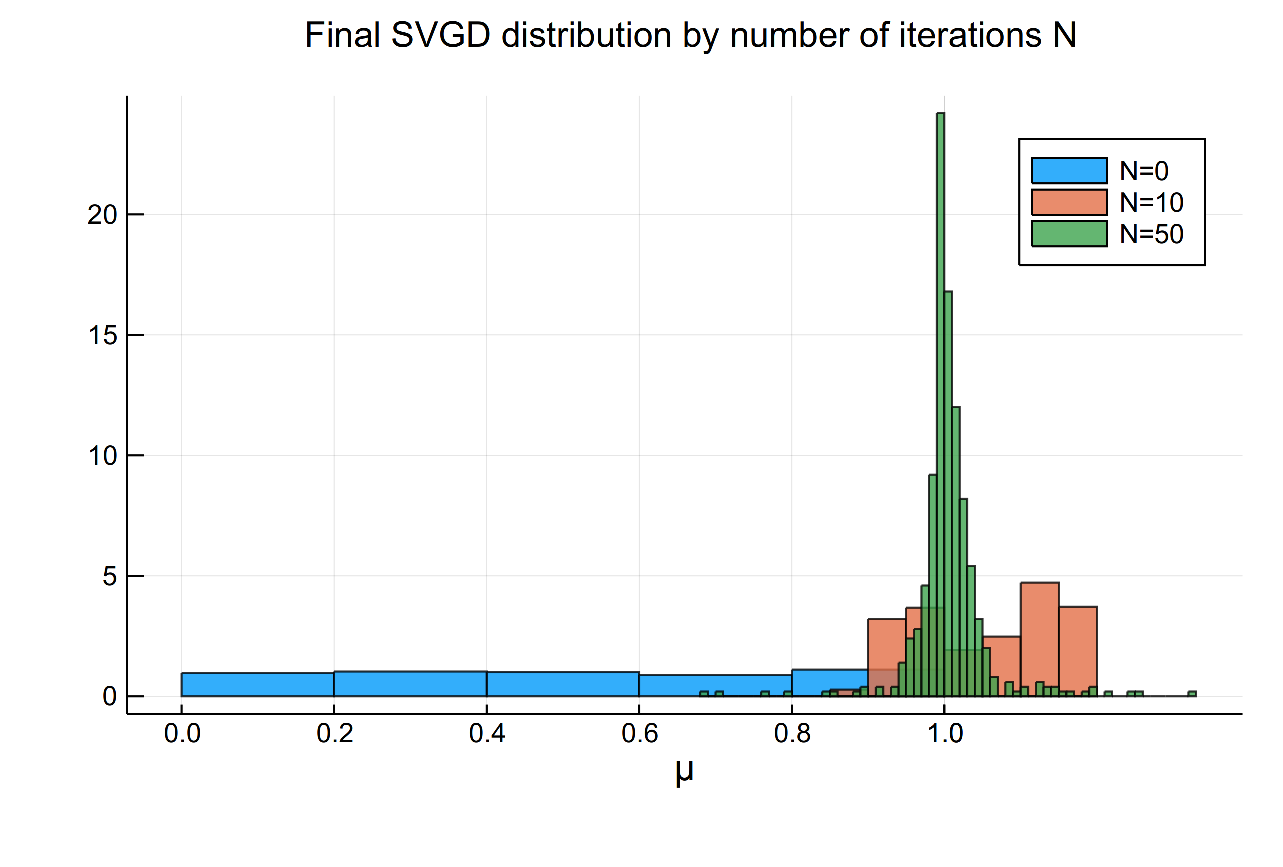
\includegraphics[width=4in]{images/svgd-example.eps}
	\caption[SVGD distribution example for different iterations.]{Graph showing how a particle distribution of 500 particles progresses towards the true parameter values of a Gaussian with mean 1. The optimisation is plotted for different amounts of iterations; the blue histogram is the initial random distribution, the green is the final result, and orange an intermediate result.}
    \label{fig:svgd-example}
\end{figure}

\begin{figure}
	\centering
	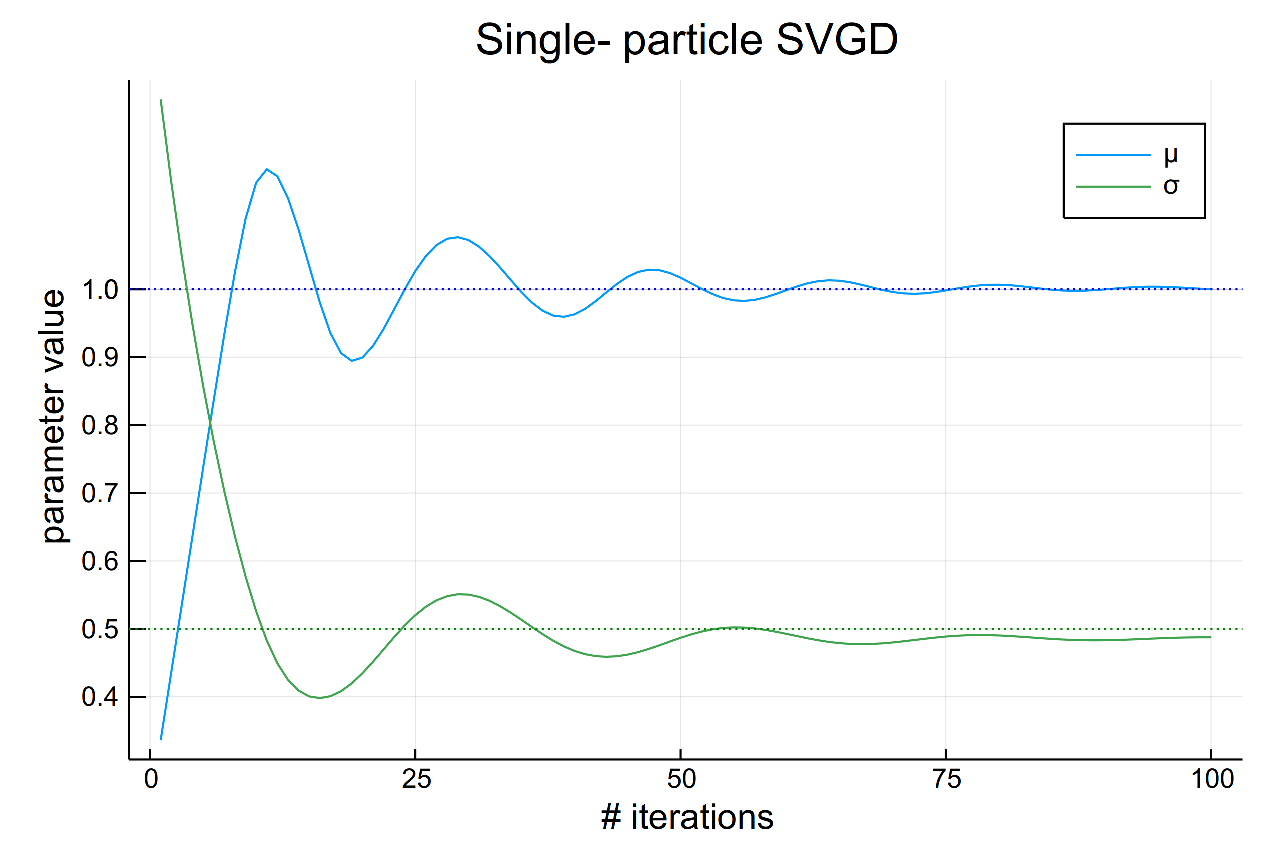
\includegraphics[width=5in]{images/svgd-map.eps}
	\caption[SVGD single-particle example graph.]{Example of the oscillating convergence of parameters $\mu$ and $\sigma$ of a Gaussian, where the dotted lines in the graph are the true parameter values. Theoretically this single-particle SVGD corresponds with MAP.}
    \label{fig:svgd-opt}
\end{figure}


\section{Comparisons of VI methods}

\subsection{Example: 1D Gaussian mixture model}
As an example we create an extremely simple Gaussian mixture model made up of two slightly overlapping normal distributions. A dataset of 1000 samples is generated with the true means $\mu_{1, 2} = (-1, 1)$ and true standard deviations $\sigma_{1, 2} = (0.3, 0.5)$.

\begin{equation}
    \begin{split}
        \mathrm{\mu}_k & \sim \mathrm{Normal}(0, 2) \\
        \sigma_k & \sim \mathrm{LogNormal}(0, 1) \\
        x_i & \sim \sum^2_{k=1} \mathrm{Normal}(\mu_k, \sigma_k) \\
    \end{split}
\end{equation}

%\begin{wrapfigure}{r}{0.5\textwidth}
\begin{figure} 
    %\begin{center}
	\centering
	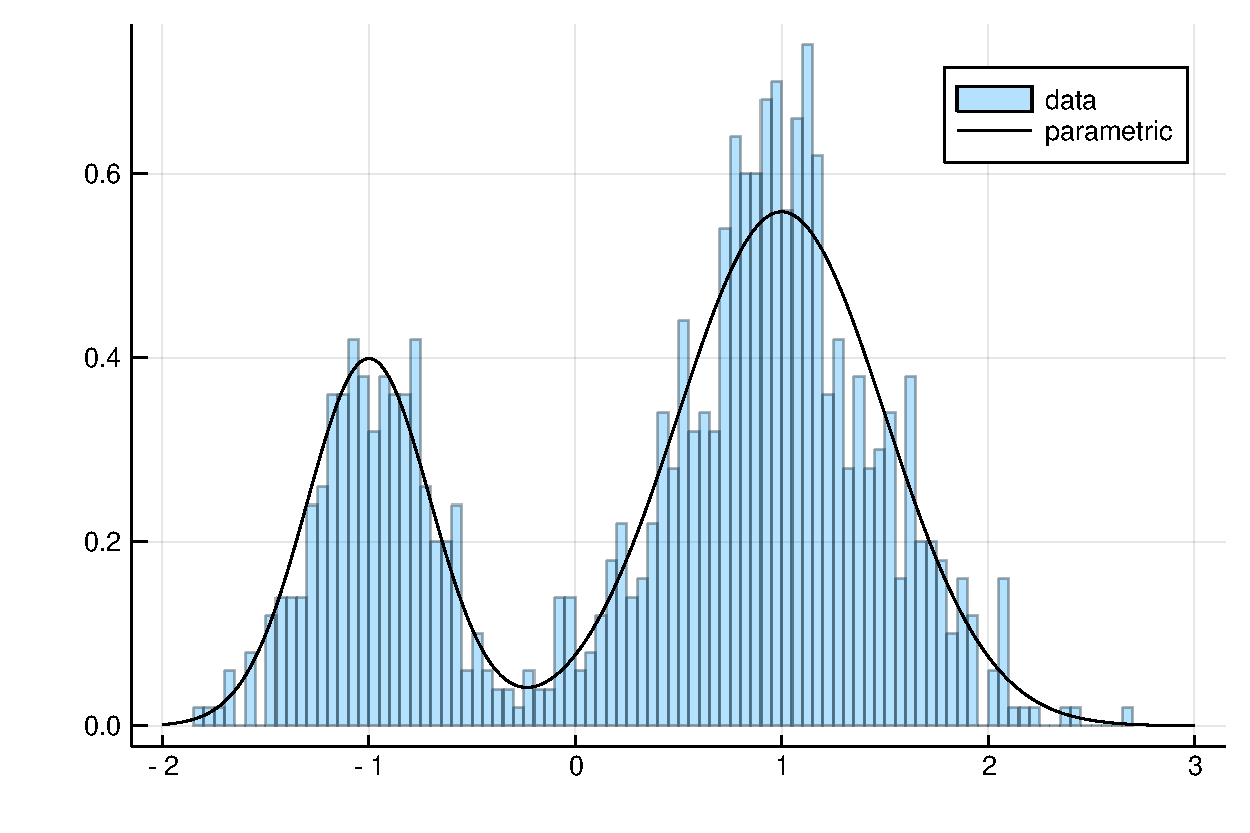
\includegraphics[width=4in]{images/vi_comp_data.pdf}
    %\end{center}
    \caption[VI comparison: true distribution of the data.]{Visualisation of the true distribution of the data samples (blue) and the parametric distribution used to generate them (black).}
    \label{fig:vi-comparison-data}
\end{figure}


    ADVI and BBVI are initialized in the same way: the initial variational distribution $q_0$ is a mean-field unit-normal distribution. Both are run for 500 iterations. 
    \\
    The 100 SVGD particles are initialized with samples from the unit normal distribution and optimised for 200 iterations. Comparison of the final distributions after optimization are visualized in Figure \ref{fig:vi-comparison}. It is clear from the graphs that all three methods find a reasonable approximation of the true values of the latent variables.
    \\ 
    In general, we note that the distributions obtained by ADVI are more narrow than the others. The parameter distributions found by SVGD are multi-modal because each particle can gravitate towards either optimum.
    

\begin{figure}
	\centering
	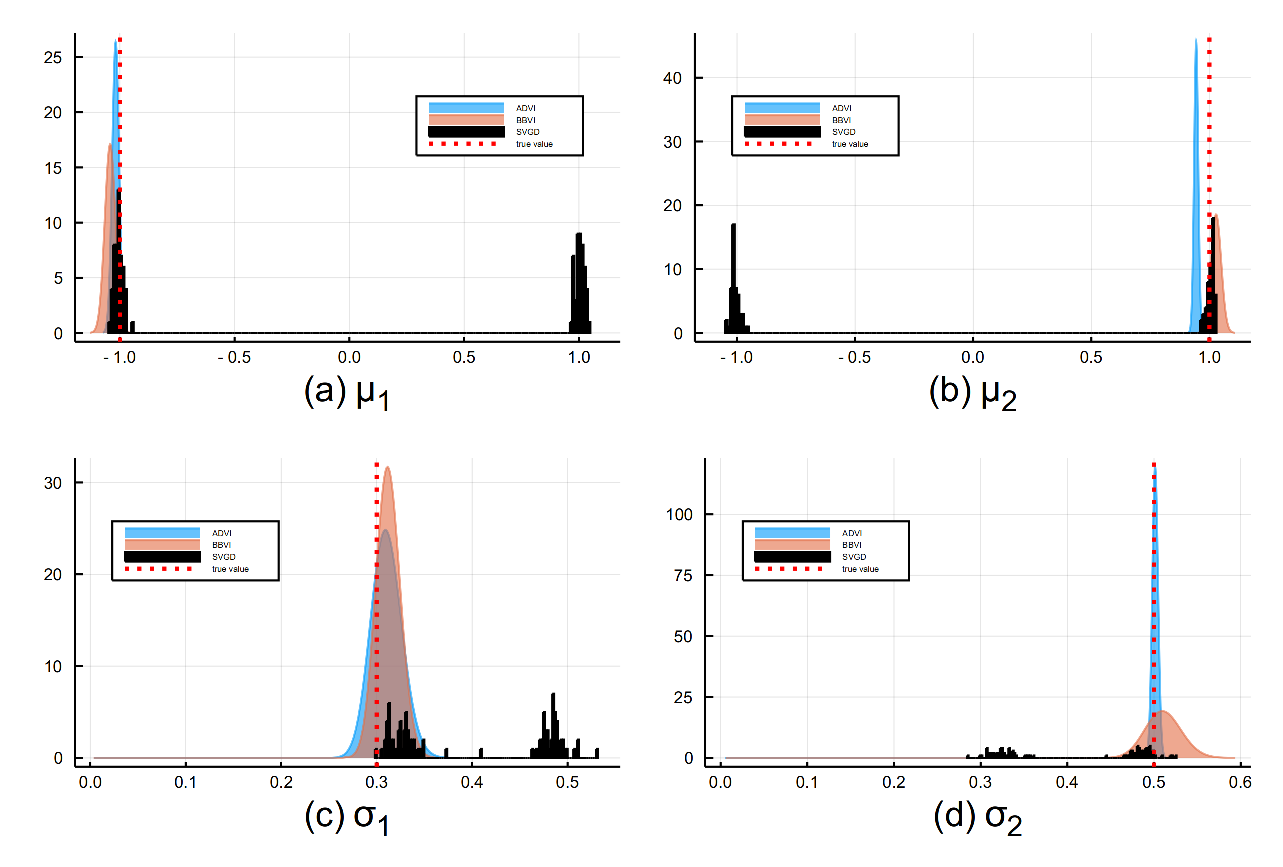
\includegraphics[width=5in]{images/vi-comp.eps}
	\caption[Comparison of densities for VI methods.]{Comparison of the inferred densities of the 1D Gaussian mixture parameters. All three methods give a reasonable approximation of the true values. Note that the results of SVGD (black) are multi-modal distributions.}
    \label{fig:vi-comparison}
\end{figure}


\subsection{Variance in gradient estimators}
BBVI and ADVI use different estimators for the gradient. Kucukelbir et al. note that the BBVI gradient estimator has much greater variance than their own ADVI method \parencite{ADVI}. When evaluating the variance for our Gaussian mixture example it is clear that this is indeed the case (see Figure \ref{fig:vi-variance}). The addition of control variates to the BBVI predictor (BBVI-CV) greatly reduces variance but it remains an order of magnitude larger than for ADVI.

\begin{figure}
	\centering
	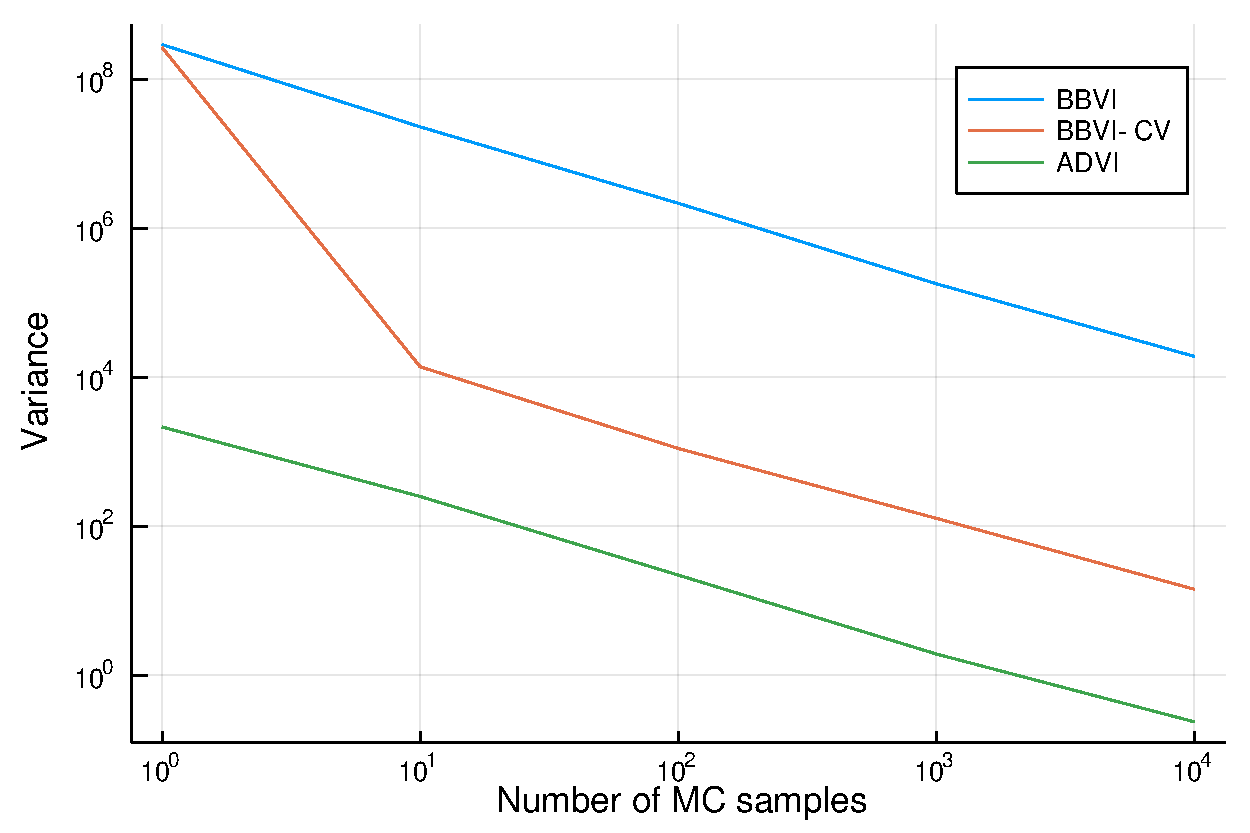
\includegraphics[width=4.2in]{images/variance_plot.pdf}
	\caption[Variance comparison of BBVI and ADVI.]{Comparison of variance on the gradient estimators of BBVI and ADVI for different amounts of Monte Carlo samples. While variance of BBVI is greatly reduced with the use of control variates (BBVI-CV), the variance of the ADVI estimator is still considerably lower.}
    \label{fig:vi-variance}
\end{figure}


\subsection{Discussion}
The results from this simple example corroborate the findings of Kucukelbir et al.: the variance of ADVI is much smaller than BBVI, resulting in much narrower peaks (Figure \ref{fig:vi-comparison}).
\\
It is also important to note that the distribution of the SVGD particles is not restricted to any variational family and that the algorithm can find multi-modal solutions when they are not expected, as in the example above. This can be useful if the shape of the distribution is completely unknown \textit{a priori}, but can make interpretation of results more difficult. An approximation that correctly estimates the mean values is often considered sufficiently accurate, which is why the mean-field normal family is most commonly used in practice \parencite{vi-review}.

\section{Variational inference in bioinformatics literature}

There have been several recent bioinformatics papers published where the authors apply variational methods to perform Bayesian inference.

\subsection{CAT model \parencite{cat}}
A variant of gradient-based variational inference called stochastic variational inference (SVI, \cite{svi}) has been successfully applied to the CAT model, which describes site heterogeneity of the nucleotide substitution process. This VI implementation proved to be up to 5x faster than MCMC and approximated the MCMC distribution accurately.

\subsection{Phylostan \parencite{phylostan}}
The \textit{phylostan} package is an extension for the probabilistic programming language Stan \parencite{Stan} that implements several common phylogenetic models. The phylostan authors opted to use the BBVI implementation already available in Stan, and compared it to the original MCMC implementation of their phylogenetic inference. They conclude that VI is much faster than MCMC, but that it is less accurate; which is what \cite{vi-review} also noted in their review paper.




